\section{The Bias Parameter}

In our analysis, we assumed $\gamma = 0$ for simplicity, but the $\gamma$ parameter
seems to be a promising knob to tune the performance of PoEM. While we leave the
analytic treatment of the optimal $\gamma$ for future work, we note here that,
for given values of $g$ and $\beta$, the delay of the system behaves as illustrated
in Figure~\ref{fig:bias} for varying values of $\gamma$. This graph behaves convexly for
small values of $\gamma$, whereas, for $\gamma \to \infty$, the delay converges to
a value smaller than Bitcoin's. Indeed, if $\gamma$ is made sufficiently large, the bias
parameter dominates against the $-\lg\frac{H(B)}{T}$ term, and the system behaves
as if each block counts the same amount of work. However, the tie-breaking rule for forks of the same
height remains, providing latency improvements still, and hence converging at the limit close to the
longest chain rule with the benefit of a tie-breaker.

\begin{figure}[h]
    \centering
    \begin{subfigure}{0.48\textwidth}
    \centering
    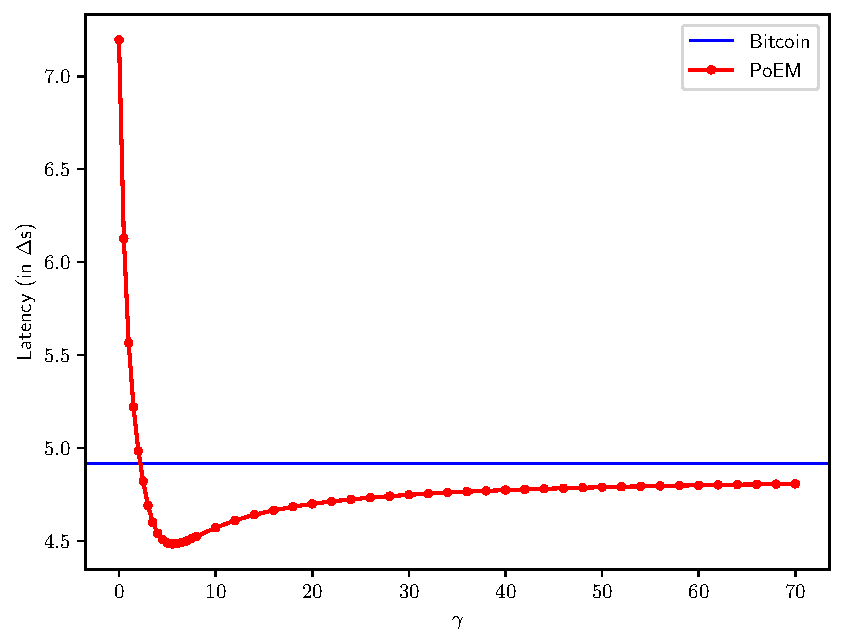
\includegraphics[width = \textwidth]{figures/gamma_latency_0.1.pdf}
    \caption{$\beta = 0.1$ and $g = 0.7$}
    \label{fig:gamma_latency_0.1}
    \end{subfigure}
    \begin{subfigure}{0.48\textwidth}
    \centering
    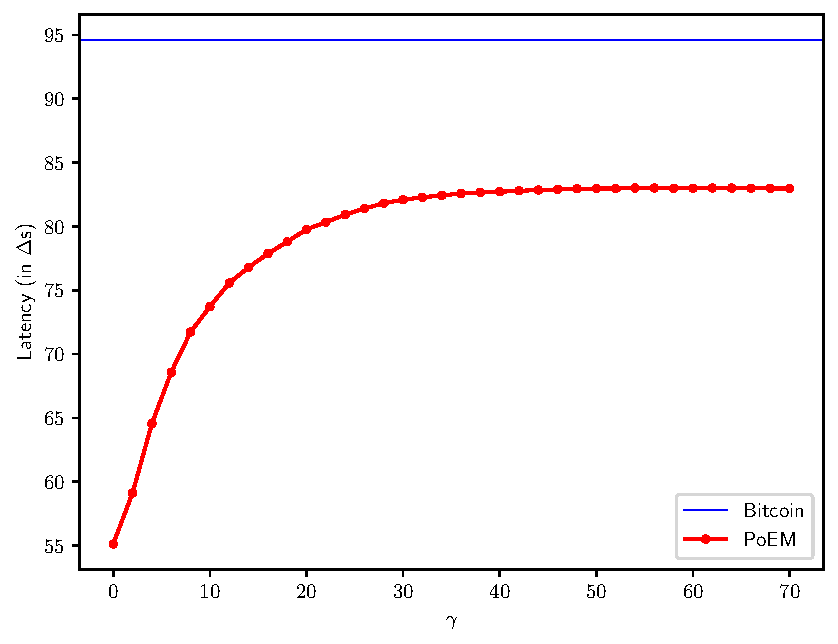
\includegraphics[width = \textwidth]{figures/gamma_latency_0.3.pdf}
    \caption{$\beta = 0.3$ and $g = 0.7$}
    \label{fig:gamma_latency_0.3}
    \end{subfigure}

  \caption{Fixing $\beta$ and $g$, we compare the latency of PoEM parameterized under different $\gamma$ values
          and the latency of Bitcoin. We observe that the plot is convex and for large $\gamma$, the latency
          converges asymptotically to a value lower than Bitcoin's latency. The results were obtained by running 100k simulations per point.}
    \label{fig:gamma_latency}
\end{figure}